\chapter{Cross-walking with fixed effects: anxiety disorder}
\label{applications-efx_study_level}

The data collected in systematic review often contain a variety of
different study types or diagnostic criteria which create systematic
biases in the measured data.  An extreme example was found in the
systematic review of diabetes prevalence, where there were $18$ variants
of diagnostic criteria.  The systematic review of anxiety disorder
provides a simpler example, which is the focus of this chapter. This
systematic review collected studies which used a handful of different
recall periods to ask about the presence of the disorder. The quantity
of interest for estimation was instantaneous prevalence, the
proportion of the population with the condition at an instant in time.
We used a fixed effect model to adjust for the bias introduced by
studies that measured past-month prevalence, since these also provide
valuable information on the descriptive epidemiology of the condition.
This bias adjustment by fixed effect modeling is also called a
``cross-walk''.

Anxiety disorders include at least eight separate conditions each
characterized by prominent anxiety at a level which interferes with
daily life.  Not all anxiety disorders manifest in similar ways.
While generalized anxiety disorder is typically marked by persistent
worry, panic disorder is usually characterized by intense fear for
discrete periods of time. \cite{association_diagnostic_2000} As there is
a lot of co-morbidity between individual anxiety disorders, anxiety
disorders are modeled together as a single condition in the GBD 2010
study.

Anxiety disorders do not have a consistent recall period for the
measurement of epidemiological rates.  Therefore the data from
systematic review have studies with measurements of point prevalence
and period prevalence (i.e. 6-month or past year prevalence).  The
analysis excludes life time prevalence as such estimates are
particularly prone to recall bias.  Due to the high remission rate for
anxiety disorders, period prevalence is typically higher than point
prevalence as seen in Figure \ref{fig:app-anxiety data}.

    \begin{figure}[h]
        \begin{center}
            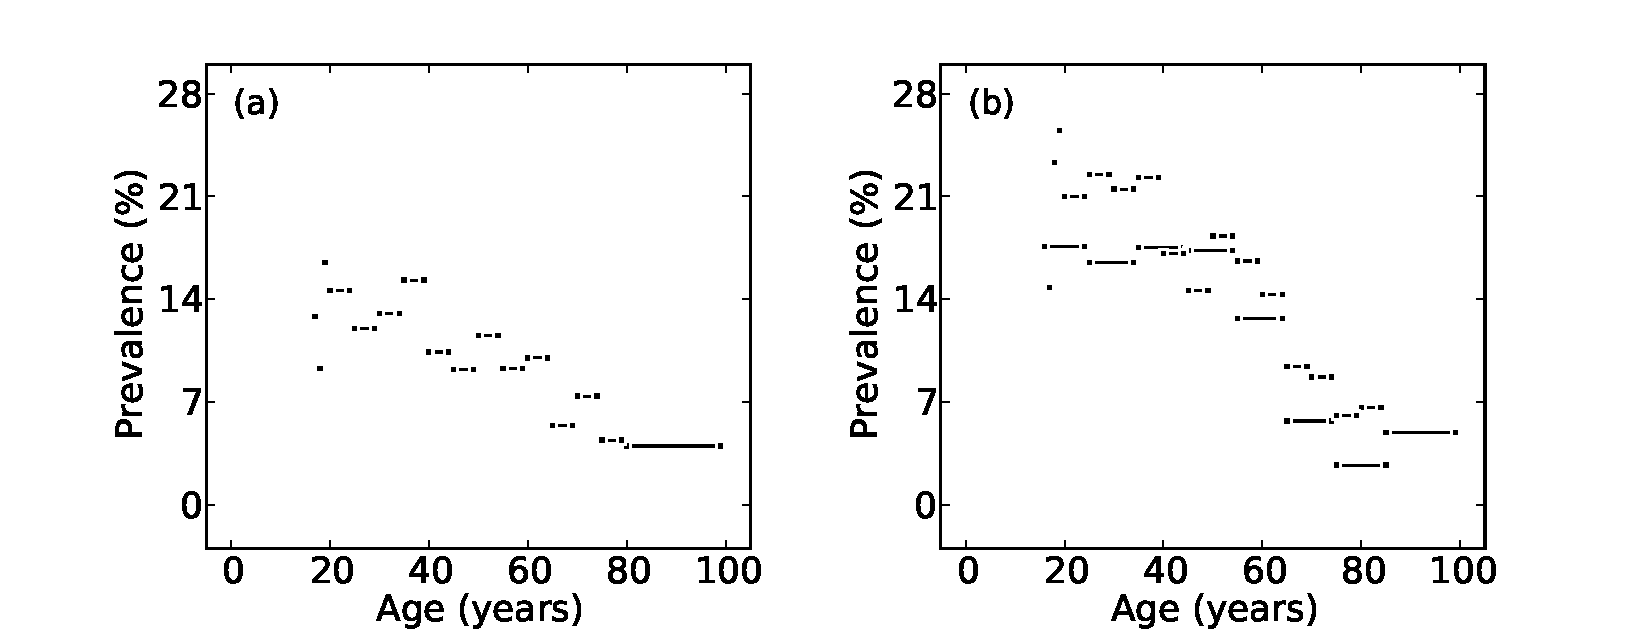
\includegraphics[width=\textwidth]{anxiety-data_by_cv.pdf}
            \caption{Point (panel (a)) and period (panel (b)) prevalence data
              for female anxiety disorders collected in systematic review for
              2000-2010 in Australasia.}
            \label{fig:app-anxiety data}
        \end{center}
    \end{figure}

Excluding period prevalence measurements reduces the quantity of data
and produces results that do not reflect the regional variation
present in the excluded data.  But including the period prevalence
measurements without a covariate to adjust for their systematic bias
leads to estimates that are noticably higher in regions where there is
data on point and period prevalence.  Using a fixed effect on a period
indicator covariate allows the model to use all available data and
explain the systematic bias and variation that results from different
recall periods, as seen in Figure \ref{fig:app-anxiety FE}.

    \begin{figure}[h]
        \begin{center}
            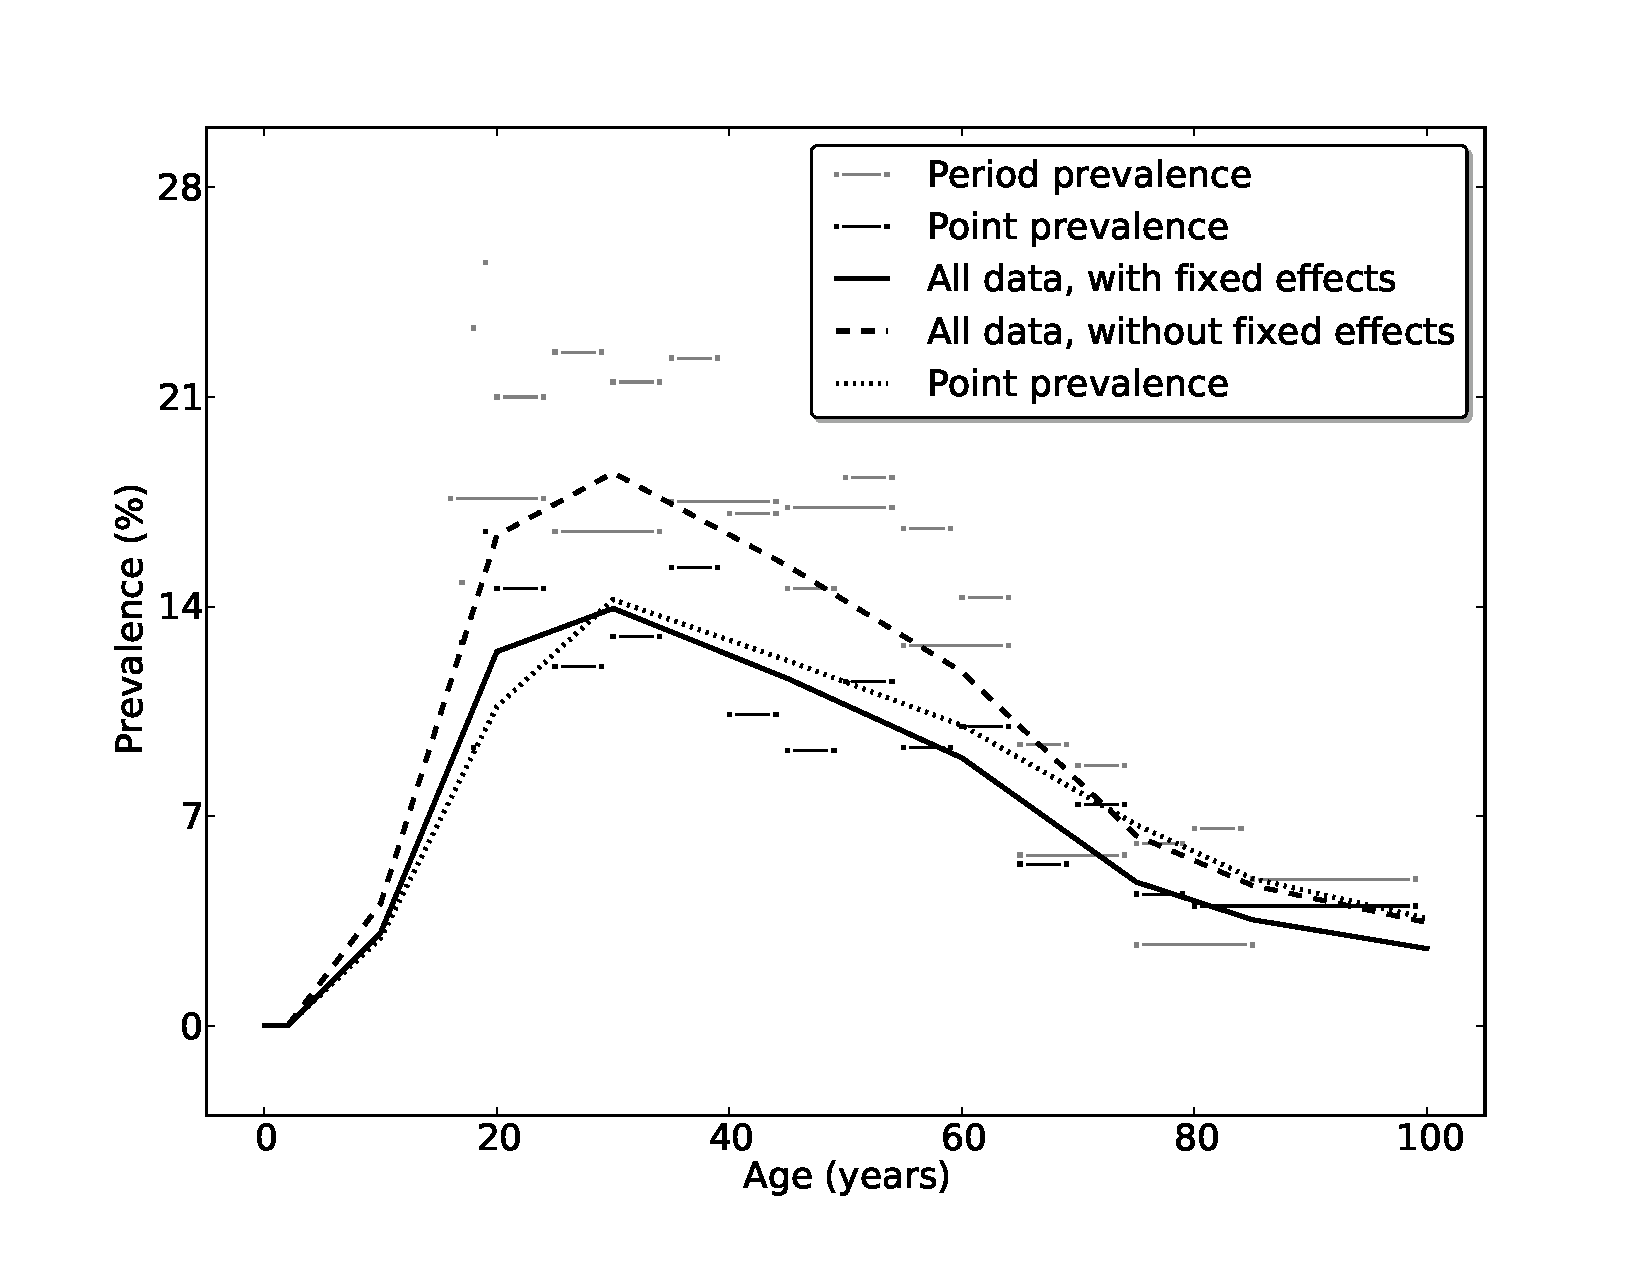
\includegraphics[width=\textwidth]{anxiety-FE.pdf}
            \caption{Comparison of prevalence estimates for anxiety
              disorders in 2005 for women in Australasia using point
              prevalence data only, point and period prevalence data
              with and without a fixed effect.}
            \label{fig:app-anxiety FE}
        \end{center}
    \end{figure}

The results of the model with a fixed effect on recall period show
that studies on period prevalence typically measure prevalence levels
49\% (95\% UI: [12, 91]) higher than if they measured point
prevalence.

A limitation of applying this method to the global dataset is that it
assumes the cross-walk factor is identical for all regions of the
world.  In practice, there is rarely enough data to move beyond this
assumption.  However, future applications may benefit from modeling
interactions between cross-walk covariates and age, sex, time, or
geography.
